\documentclass[tikz,border=3.14mm]{standalone}
\usetikzlibrary{arrows.meta,positioning}

\begin{document}
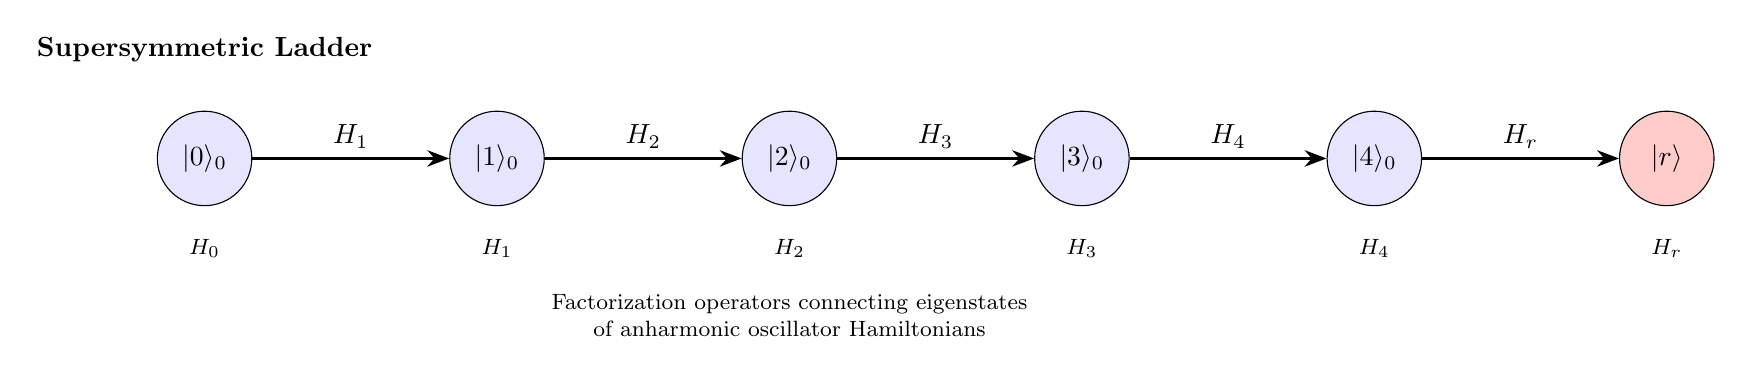
\begin{tikzpicture}[
    state/.style={circle, draw, minimum size=1.2cm, fill=blue!10},
    edge_state/.style={circle, draw, minimum size=1.2cm, fill=red!20},
    operator/.style={-{Stealth[scale=1.2]}, thick},
    node distance=2.5cm,
    label distance=2mm
]

% States of the supersymmetric ladder
\node[state] (0) {$|0\rangle_0$};
\node[state, right=of 0] (1) {$|1\rangle_0$};
\node[state, right=of 1] (2) {$|2\rangle_0$};
\node[state, right=of 2] (3) {$|3\rangle_0$};
\node[state, right=of 3] (4) {$|4\rangle_0$};
\node[edge_state, right=of 4] (r) {$|r\rangle$};

% Factorization operators connections
\draw[operator] (0) -- node[above] {$H_1$} (1);
\draw[operator] (1) -- node[above] {$H_2$} (2);
\draw[operator] (2) -- node[above] {$H_3$} (3);
\draw[operator] (3) -- node[above] {$H_4$} (4);
\draw[operator] (4) -- node[above] {$H_r$} (r);

% Hamiltonian labels
\foreach \n/\h in {0/H_0,1/H_1,2/H_2,3/H_3,4/H_4,r/H_r}
    \node[below=3mm of \n] {\footnotesize $\h$};

% Annotations
\node[above=5mm of 0, anchor=south] {\textbf{Supersymmetric Ladder}};
\node[below=10mm of 2, align=center, font=\footnotesize]
    {Factorization operators connecting eigenstates\\
     of anharmonic oscillator Hamiltonians};

\end{tikzpicture}
\end{document}